The clustered competing risks setting is a specific survival data
structure. Although, we are using a general statistical modeling
framework, a generalized linear mixed model (GLMM). Consequently, the
data structure characteristics have to be properly accommodated into the
modeling construction.

To model competing risks data we need a multivariate model and we have
to choose in which scale to work on. We may work on the hazard scale and
deal with the cause-specific hazard function or on the probability scale
and deal with the cause-specific cumulative incidence function (CIF).
By choosing the correct link function, we are able to construct an
appropriate multivariate GLMM to work on the probability scale.

Our goal is to be able to deal with complex family studies, where there
is generally a strong interest in describing age at disease onset in the
scenarios of within-cluster dependence. The distribution of age at
disease onset is directly described by the cause-specific CIF. To build
a multivariate GLMM for this type of data we need to accommodate the
cause-specific CIFs and the censorings. Assuming the conditional
distribution for our model response as multinomial we already deal with
both left-truncation and right-censoring, avoiding the specification of
a censoring distribution.  The cause-specific CIFs can be modeled via
the link function of our, then, multinomial GLMM (multiGLMM). The
multinomial distribution also guarantees that the CIFs of all causes are
modeled.

Our choice for a general framework tries to make the inference of this
complex model, easier. Besides, taking advantage of all the
computational procedures mentioned in the previous chapter. This chapter
presents our multiGLMM for clustered competing risks data and is divided
into two sections. In \autoref{cap:cif} we discuss in detail the
cluster-specific cumulative incidence function (CIF) and in
\autoref{cap:modelitself} we present the complete modeling framework.

\section{CLUSTER-SPECIFIC CUMULATIVE INCIDENCE FUNCTION (CIF)}
\label{cap:cif}

Consider that the observed follow-up time of an individual is given by
\(T = \min(T^{\ast},C)\), where \(T^{\ast}\) denote the failure time
and \(C\) denote the censoring time. Given the possible covariates
\(\bm{x}\), for a cause-specific of failure \(k\), the cumulative
incidence function (CIF) is defined as
\begin{align*}
 F_{k}(t \mid \bm{x})
 = \mathbb{P}[T \leq t,~K = k \mid \bm{x}]
 &= \int_{0}^{t} f_{k}(z \mid \bm{x})~\text{d}z\\
 &= \int_{0}^{t} \lambda_{k}(z \mid \bm{x})~S(z \mid \bm{x})
  ~\text{d}z, \quad t > 0, \quad k = 1,~\dots,~K,
\end{align*}
where \(f_{k}(t \mid \bm{x})\) is the (sub)density for the time to a
type \(k\) failure. This is the general definition of a CIF, and to
define it we need to define the functions that compose the subdensity.
The first is the cause-specific hazard function or process
\[
 \lambda_{k}(t \mid \bm{x}) = \lim_{h \rightarrow 0}~\frac{1}{h}~
 \mathbb{P}[t \leq T < t + h,~K = k \mid T \geq t,~\bm{x}],
 \quad t > 0, \quad k = 1,~\dots,~K.
\]
In words, the cause-specific hazard function \(\lambda_{k}(t \mid
\bm{x})\), represents the instantaneous rate for failures of type
\(k\) at time \(t\) given \(\bm{x}\) and all other failure types
(competing causes). If we sum up all cause-specific hazard functions we
get the overall hazard function,
\[
 \lambda(t \mid \bm{x}) = \sum_{k=1}^{K}\lambda_{k}(t \mid \bm{x}).
\]
From the overall hazard function we arrive in the overall survival
function,
\[
 S(t \mid \bm{x}) = \mathbb{P}[T > t \mid \bm{x}] =
 \exp\left\{-\int_{0}^{t} \lambda(z \mid \bm{x})~\text{d}z\right\},
\]
the second function that compose the subdensity \(f_{k}(t \mid
\bm{x})\). A comprehensive reference for all these definitions is
the book of \citeonline{kalb&prentice}.

Until this point, we were talking about a general CIF's definition. We
need now a precise framework telling us how to take into consideration
our clustered/family structure. We use the same CIF specification of
\citeonline{SCHEIKE} i.e., the approach that motivated this thesis.

For two competing causes of failure, the cause-specific CIFs are
specified in the following manner
\begin{equation}
 F_{k} (t \mid \bm{x},~u_{1},~u_{2},~\eta_{k}) =
 \underbrace{\pi_{k}(\bm{x},~u_{1},~u_{2})}_{
 \substack{\text{cluster-specific}\\\text{risk level}}}\times
  \underbrace{\Phi[w_{k} g(t) - \bm{x}\bm{\gamma}_{k} - \eta_{k}]}_{
   \substack{\text{cluster-specific}\\\text{failure time trajectory}}
  }, \quad t > 0, \quad k = 1,~2,
  \label{eq:cif}
\end{equation}
i.e., as the product of a cluster-specific risk level with a
cluster-specific failure time trajectory, resulting in a
cluster-specific CIF. What makes these components cluster-specific are
\(\bm{u} = \{u_{1},~u_{2}\}\) and \(\bm{\eta} =
\{\eta_{1},~\eta_{2}\}\), Gaussian distributed latent effects with zero
mean and potentially correlated i.e.,
\[
 \begin{bmatrix} u_{1}\\u_{2}\\\eta_{1}\\\eta_{2} \end{bmatrix} \sim
 \parbox{2.5cm}{\centering Multivariate Normal}
 \left(
  \begin{bmatrix} 0\\0\\0\\0\end{bmatrix},
  \begin{bmatrix}
   \sigma_{u_{1}}^{2}&
   \text{cov}(u_{1},~u_{2})&
   \text{cov}(u_{1},~\eta_{1})&\text{cov}(u_{1},~\eta_{2})\\
   &\sigma_{u_{2}}^{2}&
   \text{cov}(u_{2},~\eta_{1})&\text{cov}(u_{2},~\eta_{2})\\
   &&\sigma_{\eta_{1}}^{2}&\text{cov}(\eta_{1},~\eta_{2})\\
   &&&\sigma_{\eta_{2}}^{2}
  \end{bmatrix}
 \right).
\]
The cluster-specific survival function is given by \(S(t \mid
\bm{x},~\bm{u},~\bm{\eta}) = 1 - F_{1} (t \mid
\bm{x},~\bm{u},~\eta_{1}) - F_{2} (t \mid
\bm{x},~\bm{u},~\eta_{2})\). Since we use the same CIF specification
of \citeonline{SCHEIKE}, the following details are essentially the same
encountered in the paper.

Focusing first on the second component of \autoref{eq:cif}, the
cluster-specific failure time trajectory
\[
 \Phi[w_{k} g(t) - \bm{x}\bm{\gamma}_{k} - \eta_{k}],
 \quad t > 0, \quad k = 1,~2,
\]
where \(\Phi(\cdot)\) is the cumulative distribution function of a
standard Gaussian distribution. Instead of \(w_{k} g(t)\), in
\citeonline{SCHEIKE} is specified \(\alpha_{k}(g(t))\) with
\(\alpha_{k}(\cdot)\) being a monotonically increasing function known up
to a finite-dimensional parameter vector, \(w_{k}\). Examples are
monotonically increasing B-splines or piecewise linear functions.
However, to simplify the model structure we consider just the
finite-dimensional parameter vector. The bottom line is that the authors
do the same approach in their applications. With regard to the function
\(g(t)\), it plays a crucial role since the CIF separation in
\autoref{eq:cif} is only possible with it. It is used a time \(t\)
transformation given by
\[
 g(t) = \text{arctanh}\left(\frac{t - \delta/2}{\delta/2}\right),
 \quad t\in(0,~\delta), \quad g(t)\in(-\infty,~\infty),
\]
where \(\delta\) depends on the data and cannot exceed the maximum
observed follow-up time \(\tau\) i.e., \(\delta \leq \tau\). With this
Fisher-based transformation the value of the cluster-specific failure
time trajectory is equal 1, at time \(\delta\). Consequently, \(F_{k}
(\delta \mid \bm{x},~\bm{u},~\eta_{k}) = \pi_{k}(\bm{x} \mid
\bm{u})\) and we can interpret \(\pi_{1}(\bm{x} \mid \bm{u})\) and
\(\pi_{2}(\bm{x} \mid \bm{u})\) as the cause-specific
cluster-specific risk levels, at time \(\delta\).

The cluster-specific risk levels are modeled by a multinomial logistic
regression model with latent effects i.e.,
\begin{equation}
 \pi_{k}(\bm{x}, \bm{u}) =
 \frac{\exp\{\bm{x}\bm{\beta}_{k} + u_{k}\}}{1 +
  \exp\{\bm{x}\bm{\beta}_{1} + u_{1}\} +
  \exp\{\bm{x}\bm{\beta}_{2} + u_{2}\}}, \quad k = 1,~2,
 \label{eq:risklevel}
\end{equation}
where the \(\bm{\beta}_{k}\)'s are the coefficients responsible for
quantifying the impact of the covariates in the cause-specific risk
levels. For individuals from the same chuster/family, at the same time
point, the \(\bm{\beta}_{k}\)s have the well-known odds ratio
interpretation.

A direct understanding of all coefficients/parameters of
\autoref{eq:cif} can be reached via the illustrations in
\autoref{fig:cifcoefs}. To really understand what is going on, we
simplify the model. We still consider just two competing causes but
without covariates and we plot just the cluster-specific CIF of one
failure cause. In \autoref{fig:cifcoefs}~A) we see that the \(\beta\)'s
are also related with the curve's maximum value i.e., bigger the
\(\beta\), highest the CIF will be.

The \(\bm{\gamma}_{k}\)'s are the coefficients responsible for
quantifying the impact of the covariates in the cause-specific failure
time trajectories i.e., the shape of the cumulative incidence. In
\autoref{fig:cifcoefs}~B) we see that the \(\gamma\)'s are also related
with an idea of midpoint and consequently, growth speed. The fact that
\(\gamma_{k}\) enters negatively in the cluster-specific failure time
trajectory makes that a negative value causes an advance towards the
curve, whereas a positive value causes a delay. Last but not least, the
\(w\)'s in \autoref{fig:cifcoefs}~C). With negative values, we have a
decreasing curve and with positive values an increasing curve i.e., we
are interested only on the positive side.

\begin{figure}[H]
 \setlength{\abovecaptionskip}{.0001pt}
 \caption{ILLUSTRATION OF COEFFICIENT BEHAVIORS FOR A GIVEN CUMULATIVE
          INCIDENCE FUNCTION (CIF) (PROPOSED BY \citeonline{SCHEIKE}),
          IN A MODEL WITH TWO COMPETING CAUSES OF FAILURE, WITHOUT
          COVARIATES, AND WITH THE FOLLOWING CONFIGURATION: \(\beta_{2}
          = 0\), \(\bm{u} = 0\) AND \(\bm{\eta} = 0\); IN EACH SCENARIO
          ALL OTHER COEFFICIENTS ARE SET TO ZERO, WITH THE EXCEPTION
          OF \(w_{1} = 1\)}
 \vspace{0.2cm}\centering
 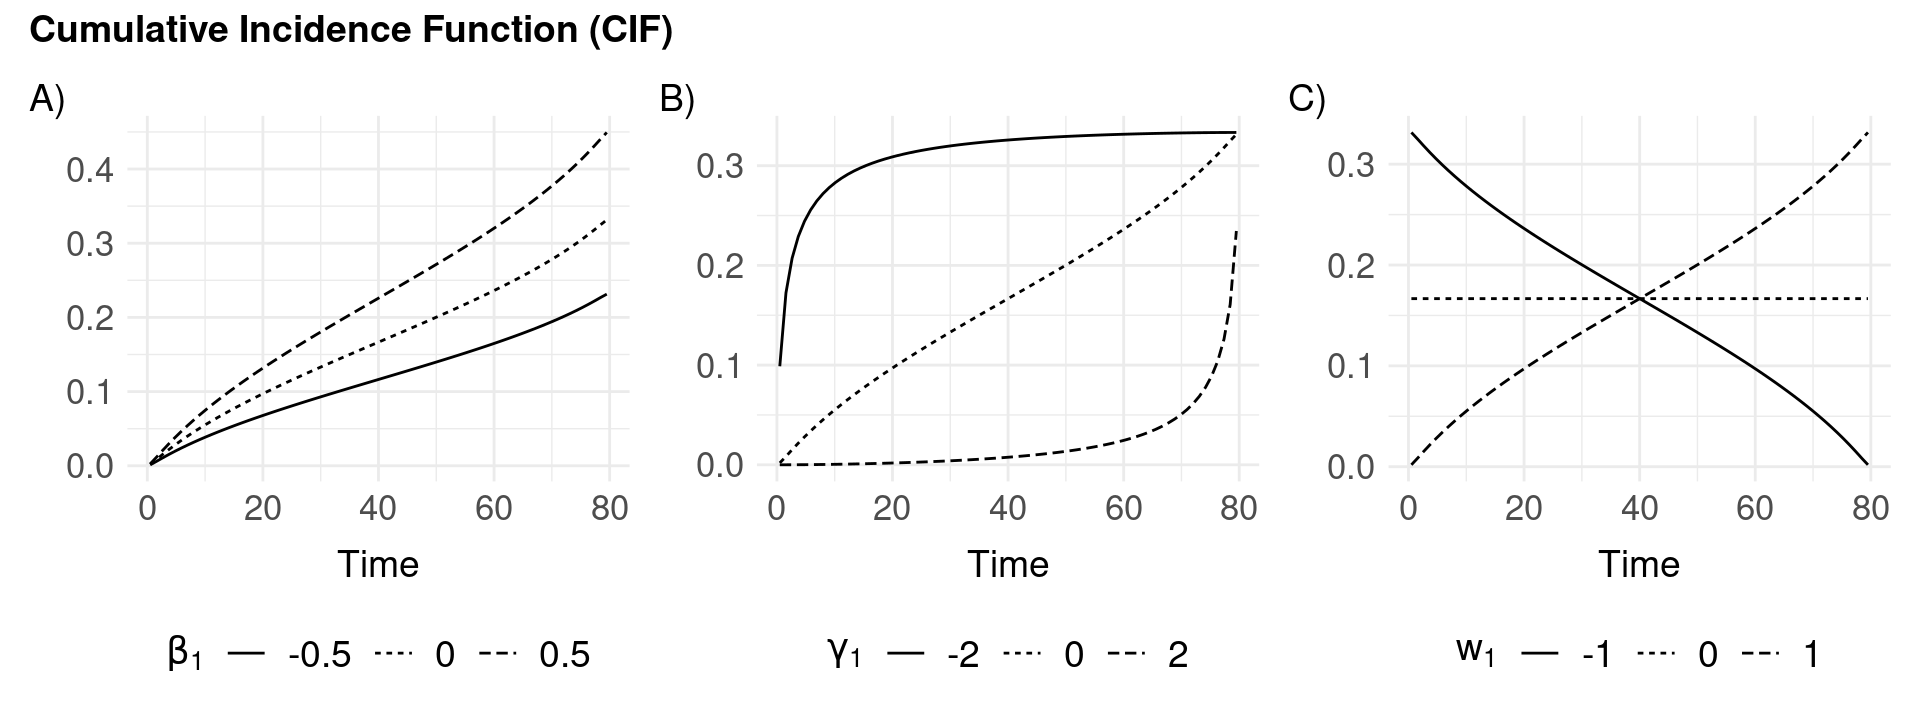
\includegraphics[width=\textwidth]{cifcoefs-1.png}\\
 \begin{footnotesize}
  SOURCE: The author (2021).
 \end{footnotesize}
 \label{fig:cifcoefs}
\end{figure}

Remains to talk about the within-cluster dependence induced by the
latent effects in \(\bm{u}\) and \(\bm{\eta}\). Unfortunately, they do
not have an easy interpretation. To help in the discussion,
\autoref{fig:cif} illustrates the cluster-specific CIF for a given
failure cause in a model without covariates, let us call it failure
cause 1 (in total we have two).

The latent effects \(u_{1}\) and \(u_{2}\) always appear together in the
cluster-specific risk level, as consequency they have a joint effect on
the cumulative incidence of both causes. As we can see in
\autoref{fig:cif}, an increase in \(u_{k}\) will increase the risk of
failure from cause \(k\). The interpretation of
\(\text{cov}(\eta_{1},~\eta_{2})\) and \(\text{cov}(u_{1},~u_{2})\) is
straightforward, and those values are in most of the cases positive, as
said in \citeonline{SCHEIKE}. With regard to
\(\text{cov}(u_{k},~\eta_{k})\), negative values are the common
situation. A negative correlation between \(\eta_{k}\) and \(u_{k}\)
imply that when \(\eta_{k}\) decreases, \(u_{k}\) increases and
conversely when \(\eta_{K}\) increases, \(u_{k}\) decreases. In other
words, an increased risk level is reached quickly and a decreased risk
level is reached later, respectively.

Practical situations with a positive within-cause correlation are hard
to find i.e., where an increased risk level is associated with a late
onset and vice versa. However, a positive cross-cause correlation
between \(\eta\) and \(u\) sounds much more realistic i.e., where late
onset of one failure cause is associated with a high absolute risk of
another failure cause.

\begin{figure}[H]
 \setlength{\abovecaptionskip}{.0001pt}
 \caption{ILLUSTRATION OF A GIVEN CLUSTER-SPECIFIC CUMULATIVE INCIDENCE
          FUNCTION (CIF), PROPOSED BY \citeonline{SCHEIKE}, IN A MODEL
          WITH TWO COMPETING CAUSES OF FAILURE, WITHOUT COVARIATES AND
          THE FOLLOWING CONFIGURATION: \(\beta_{1} = -2\),
          \(\beta_{2} = -1\), \(\gamma_{1} = 1\), \(w_{1} = 3\) AND
          \(u_{2} = 0\). THE VARIATION BETWEEN FRAMES IS GIVEN BY THE
          LATENT EFFECTS \(u_{1}\) AND \(\eta_{1}\)}
 \vspace{0.2cm}\centering
 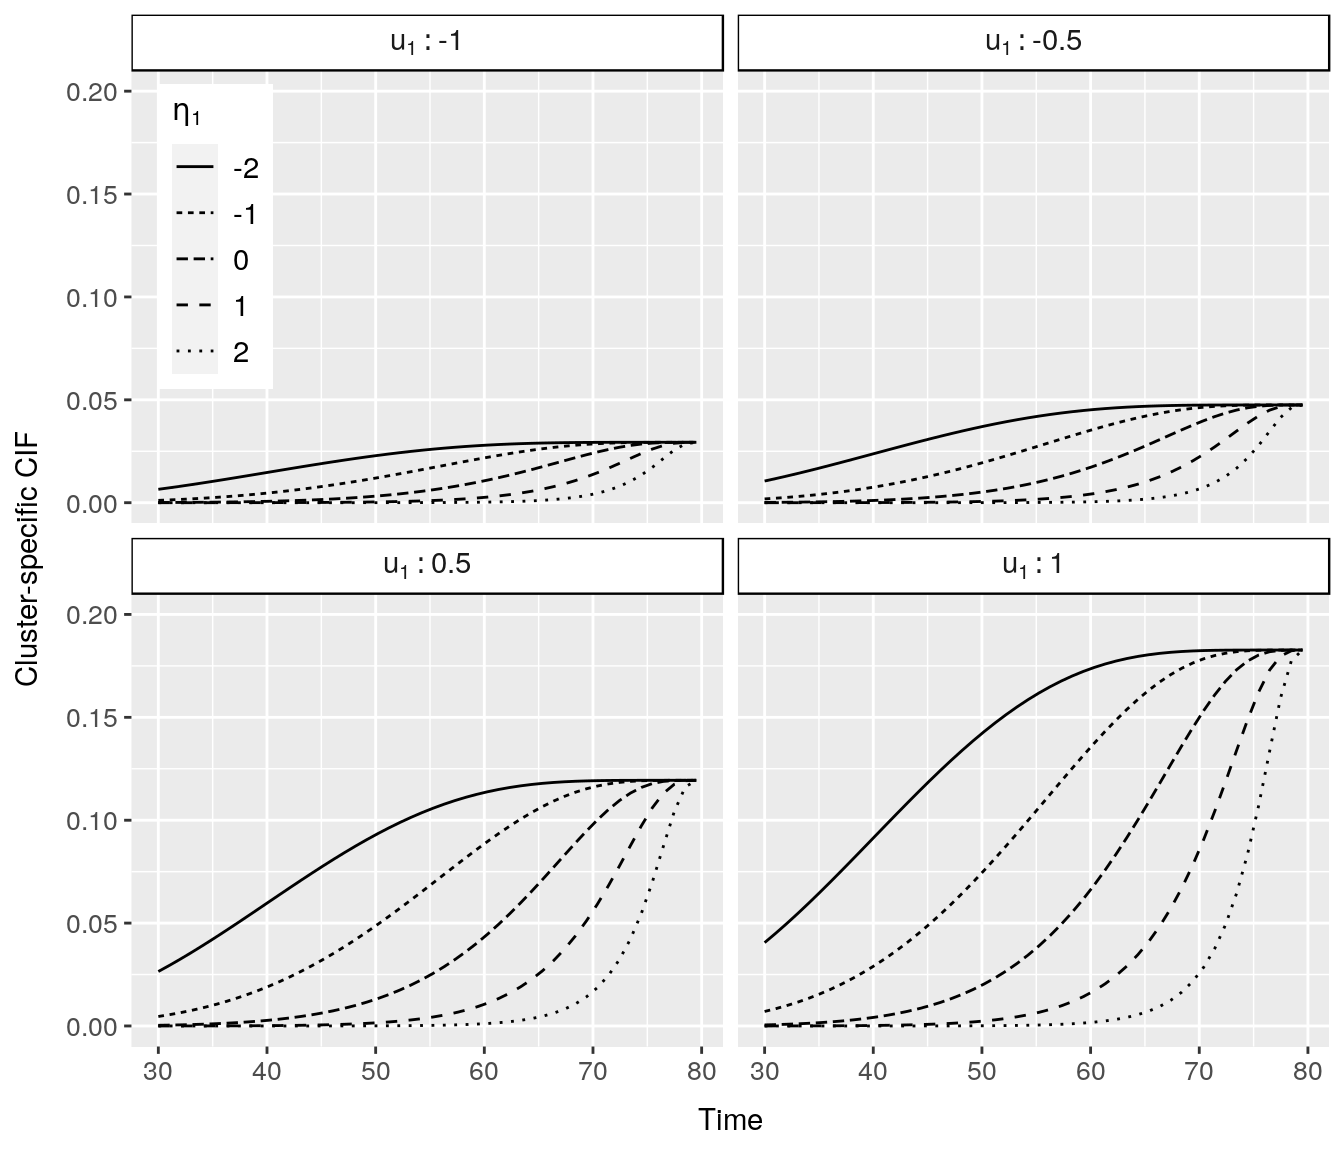
\includegraphics[width=0.9\textwidth]{cif-1.png}\\
 \begin{footnotesize}
  SOURCE: The author (2021).
 \end{footnotesize}
 \label{fig:cif}
\end{figure}

The latent effects \(\{u_{k},~\eta_{k}\}\) are assumed independent
across clusters and shared by individuals within the same
cluster/family.

\section{MODEL SPECIFICATION}
\label{cap:modelitself}

The multiGLMM for clustered competing risks data is specified in the
following hierarchical fashion. By simplicity, we focus on two competing
causes of failure but an extension is straightforward.

For two competing causes of failure, a subject \(i\), in the
cluster/family \(j\), in time \(t\), we have
\begin{align}
 y_{i j t} \mid \{u_{1j},~u_{2j},~\eta_{1j},~\eta_{2j}\}
 &\sim\text{Multinomial}(p_{1ijt},~p_{2ijt},~p_{3ijt})\nonumber\\
 \nonumber\\
 \begin{bmatrix} u_{1}\\u_{2}\\\eta_{1}\\\eta_{2} \end{bmatrix}
 &\sim\text{MN}
  \left(
   \begin{bmatrix} 0\\0\\0\\0 \end{bmatrix},
   \begin{bmatrix}
    \sigma_{u_{1}}^{2}&
    \text{cov}(u_{1},~u_{2})&
    \text{cov}(u_{1},~\eta_{1})&\text{cov}(u_{1},~\eta_{2})\\
    &\sigma_{u_{2}}^{2}&
    \text{cov}(u_{2},~\eta_{1})&\text{cov}(u_{2},~\eta_{2})\\
    &&\sigma_{\eta_{1}}^{2}&\text{cov}(\eta_{1},~\eta_{2})\\
    &&&\sigma_{\eta_{2}}^{2}
   \end{bmatrix}
  \right)\nonumber\\
 \nonumber\\
 p_{kijt}
 &=\frac{\partial}{\partial t}
  F_{k} (t \mid \bm{x},~u_{1},~u_{2},~\eta_{k})\label{eq:model}\\
 &= \frac{\exp\{\bm{x}_{kij}\bm{\beta}_{k} + u_{kj}\}}{
    1 + \sum_{m=1}^{K-1}\exp\{\bm{x}_{mij}\bm{\beta}_{m} + u_{mj}\}}
  \nonumber\\
 &\times w_{k}\frac{\delta}{2\delta t - 2t^{2}}~
  \phi\left(
   w_{k}
   \text{arctanh}\left(\frac{t-\delta/2}{\delta/2}\right)
   - \bm{x}_{kij}\bm{\gamma}_{k} - \eta_{kj}
  \right),\nonumber\\k = 1,~2.\nonumber
\end{align}
The probabilities are given by the derivative w.r.t. time \(t\) of the
cluster-specific CIF. The choice of a multinomial logistic regression
model ensures that the sum of the predicted cause-specific CIFs does not
exceed 1.

Considering two competing causes of failure, we have a multinomial with
three classes. The third class exists to handle the censorship and its
probability is given by the complementary to reach 1. This framework in
\autoref{eq:model} results in what we call multiGLMM, a multinomial
GLMM to handle the CIF of clustered competing risks data. For a random
sample, the corresponding marginal likelihood functions in given by
\begin{align}
 L(\bm{\theta}~;~y)
 &= \prod_{j=1}^{J}~\int_{\Re^{4}}
    \pi(y_{j} \mid \bm{r}_{j})\times\pi(\bm{r}_{j})~\text{d}\bm{r}_{j}
    \nonumber\\
 &= \prod_{j=1}^{J}~\int_{\Re^{4}}
    \Bigg\{
    \underbrace{\prod_{i=1}^{n_{j}}~\prod_{t=1}^{n_{ij}}
    \Bigg(
    \frac{(\sum_{k=1}^{K}y_{kijt})!}{y_{1ijt}!~y_{2ijt}!~y_{3ijt}!}~
    \prod_{k=1}^{K} p_{kijt}^{y_{kijt}}
    \Bigg)}_{\substack{\text{fixed effect component}}}
  \Bigg\}\times\nonumber\\
 &\hspace{2cm}\underbrace{
   (2\pi)^{-2} |\Sigma|^{-1/2} \exp
   \left\{-\frac{1}{2}\bm{r}_{j}^{\top} \Sigma^{-1} \bm{r}_{j}\right\}
   }_{\substack{\text{latent effect component}}}
   \text{d}\bm{r}_{j}\nonumber\\
 &= \prod_{j=1}^{J}~\int_{\Re^{4}}
    \Bigg\{
    \underbrace{\prod_{i=1}^{n_{j}}~\prod_{t=1}^{n_{ij}}
    \prod_{k=1}^{K} p_{kijt}^{y_{kijt}}
    }_{\substack{\text{fixed effect}}}
   \Bigg\}\underbrace{
   (2\pi)^{-2} |\Sigma|^{-1/2} \exp
   \left\{-\frac{1}{2}\bm{r}_{j}^{\top} \Sigma^{-1} \bm{r}_{j}\right\}
   }_{\substack{\text{latent effect component}}}
   \text{d}\bm{r}_{j}\label{eq:loglik},
\end{align}
where \(\bm{\theta} = [\bm{\beta}~\bm{\gamma}~\bm{w}~\bm{\sigma^{2}}~
\bm{\rho}]^{\top}\) is the parameters vector to be maximized. In our
framework, a subject can fail from just one competing cause or get
censor, at a given time. Thus, the fraction of factorials in the fixed
effect component is made only by 0's and 1's. Finally, returning the
value 1. The matrix \(\Sigma\) is the variance-covariance matrix, which
parameters are given by \(\bm{\sigma}^{2}\) and \(\bm{\rho}\).

Now, \autoref{eq:loglik} in words. To each cluster/family \(j\) we have
a product of two components. The fixed effect component, given by a
multinomial distribution with its probabilities specified through the
cluster-specific CIF (\autoref{eq:cif}) and, the latent effect
component, given by a multivariate Gaussian distribution.

To each subject \(i\) that composes a cluster \(j\) we have its specific
fixed effects contribution. The likelihood in \autoref{eq:loglik} is the
most general as possible, allowing for repeated measures to each
subject. Since all subjects of a given cluster shares the same latent
effect, we have just one latent effect contribution multiplying the
product of fixed effect contributions. As we do not observe the latent
effect variables, \(\bm{r}_{j}\), we integrate out in it. With two
competing causes of failure, we have four latent effects (a multivariate
Gaussian distribution in four dimensions). Consequently, for each
cluster, we approximate an integral in four dimensions. The product of
these approximated integrals results in the called marginal likelihood,
to be maximized in \(\bm{\theta}\).

Independent of the parameters value choice, the probabilities for the
failure causes will be small, providing always a bigger probability mass
to the censorship. More will be talked about this model characteristic
in the next chapter.

\subsection{Parametrization}
\label{cap:parametrization}

We have to choose in which terms we parameterize the variance-covariance
matrix \(\Sigma\). Besides the latent effects variances
\(\{\bm{\sigma^{2}}\}\), we have to choose if we will estimate its
covariances or correlations. By the name \textit{variance-covariance}
matrix, it is natural to think on covariance terms. However, this option
is not very attractive since its interpretation is not clear. A more
attractive choice is in terms of correlation.

The covariance between two terms is defined as a triple product: the two
terms standard deviations times the correlation, \(\rho\). Still
thinking in two competing causes of failure, we have an \(\Sigma\)
matrix with six correlations
\begin{align*}
 \Sigma = \begin{bmatrix}
           \sigma_{u_{1}}^{2}&
           \rho_{u_{1},u_{2}}~\sigma_{u_{1}}\sigma_{u_{2}}&
           \rho_{u_{1},\eta_{1}}~\sigma_{u_{1}}\sigma_{\eta_{1}}&
           \rho_{u_{1},\eta_{2}}~\sigma_{u_{1}}\sigma_{\eta_{2}}\\
           &\sigma_{u_{2}}^{2}&
           \rho_{u_{2},\eta_{1}}~\sigma_{u_{2}}\sigma_{\eta_{1}}&
           \rho_{u_{2},\eta_{2}}~\sigma_{u_{2}}\sigma_{\eta_{2}}\\
           &&\sigma_{\eta_{1}}^{2}&
           \rho_{\eta_{1},\eta_{2}}~\sigma_{\eta_{1}}\sigma_{\eta_{2}}\\
           &&&\sigma_{\eta_{2}}^{2}
          \end{bmatrix}.
\end{align*}
With the matrix parametrization being chosen, we have that the
parameters to be estimated are the components of the vector
\(\bm{\theta} = [\bm{\beta}~ \bm{\gamma}~\bm{w}~\bm{\sigma^{2}}~
\bm{\rho}]^{\top}\). There we have the fixed effects or mean components
\(\{\bm{\beta}~\bm{\gamma}~\bm{w}\}\), the easiest to estimate in a
statistical modeling framework; we have variance components
\(\{\bm{\sigma^{2}}\}\), the intermediate ones; and the correlation
components \(\{\bm{\rho}\}\), the hardest ones. This idea of easy or
hard to estimate may be justified by three, connected, arguments.

The first comes from the fact that we are modeling the mean of a
probability distribution in a hierarchical and structured fashion,
consequently, the easiest parameters to estimate will be the mean
components. We may make the analogy that to estimate the mean parameters
we need data (resources); to estimate the variance parameters we need
more data (more resources), and to estimate the correlation parameters
we need much more data (even more resources). The second argument comes
to also explain the first one via the parametric space constraints.

Generally, the fixed effect components do not present constraints, i.e.
they can vary in all \(\mathbb{R}\). The same can not be said from the
variance components, constrained by definition into the
\(\mathbb{R}_{\ast}^{+}\). Finally, we have the correlation components,
constrained to the interval \([-1,~1]\). These parametric space
constraints drive us again to the first argument since we need more data
(resources, information) to be able to estimate coefficients constrained
to some interval. Nevertheless, this may not be enough. Without
providing some extra information, in terms of an constrained algorithm
e.g., it is very reasonable to expect that during the optimization
procedure some unrealistic areas of the parametric space could be
visited and jeopardize the stability or even the whole optimization
procedure. To overcome these possible difficulties, parameter
reparametrizations are more than welcome.

The variance and correlation parameters are modeled in terms of the
matrix \(\Sigma\). This matrix is symmetric and more important, positive
semi-definite. This last characteristic is also the third argument to
justify why is so difficult to estimate these parameters. Since the
estimates should lead to a positive semi-definite matrix, the employment
of a parametrization is welcome to enforces this condition.

In the subject of choosing the components parametrization for a
positive-definite matrix \(\Sigma\), we have basically two big options
available in the statistical modeling literature. One of them consists
of just transform the scale. By practical reasons, let us think in a
\(2\times 2\) matrix
\begin{align*}
 \Sigma = \begin{bmatrix}
           \exp\{\log\sigma_{1}^{2}\}&
           z^{-1}(z(\rho_{1,2}))
           \sqrt{\exp\{\log\sigma_{1}^{2}\}}
           \sqrt{\exp\{\log\sigma_{1}^{2}\}}\\
           &\exp\{\log\sigma_{2}^{2}\}
          \end{bmatrix},
\end{align*}
i.e. in the main diagonal we now estimate the log variances and in the
off-diagonal we estimate Fisher z-transformed correlations.

The estimation of the log variances has two big advantages
\begin{itemize}
 \item Since the natural lorarithm is a real-valued function, we
       overcome the parametric space constraint problem;
 \item High variances are problematic for many reasons but in the
       context of seeing them as the diagonal components of a restricted
       matrix, being able to control its magnitudes is a crucial task to
       the stability of any optimization routine. With the natural
       logarithm transformation we shrink the parametric space, as
       illustrated in \autoref{fig:parametrization}~A), avoiding some
       eventual numerical cumbersome.
\end{itemize}
With the correlation components what we do is to proceed with the
estimation of its Fischer z-transformation. This transformation, and its
inverse, are defined as
\[
 z(\rho) = \frac{1}{2}\log\Big(\frac{1+\rho}{1-\rho}\Big)
         = \text{arctanh}(\rho),\quad
 z^{-1}(\rho) = \frac{\exp\{2\rho\}-1}{\exp\{2\rho\}+1}
             = \text{tanh}(\rho).
\]
The Fisher z-transformation plays the role here of stretching the small
correlation parametric space but doing this in a smooth fashion, as
illustrated in \autoref{fig:parametrization}~B).

\begin{figure}[H]
 \setlength{\abovecaptionskip}{.0001pt}
 \caption{ILLUSTRATION OF THE PARAMETRIZATION BEHAVIOR FOR THE VARIANCE
          COMPONENTS, IN A), AND CORRELATION COMPONENTS, IN B)}
 \vspace{0.3cm}\centering
 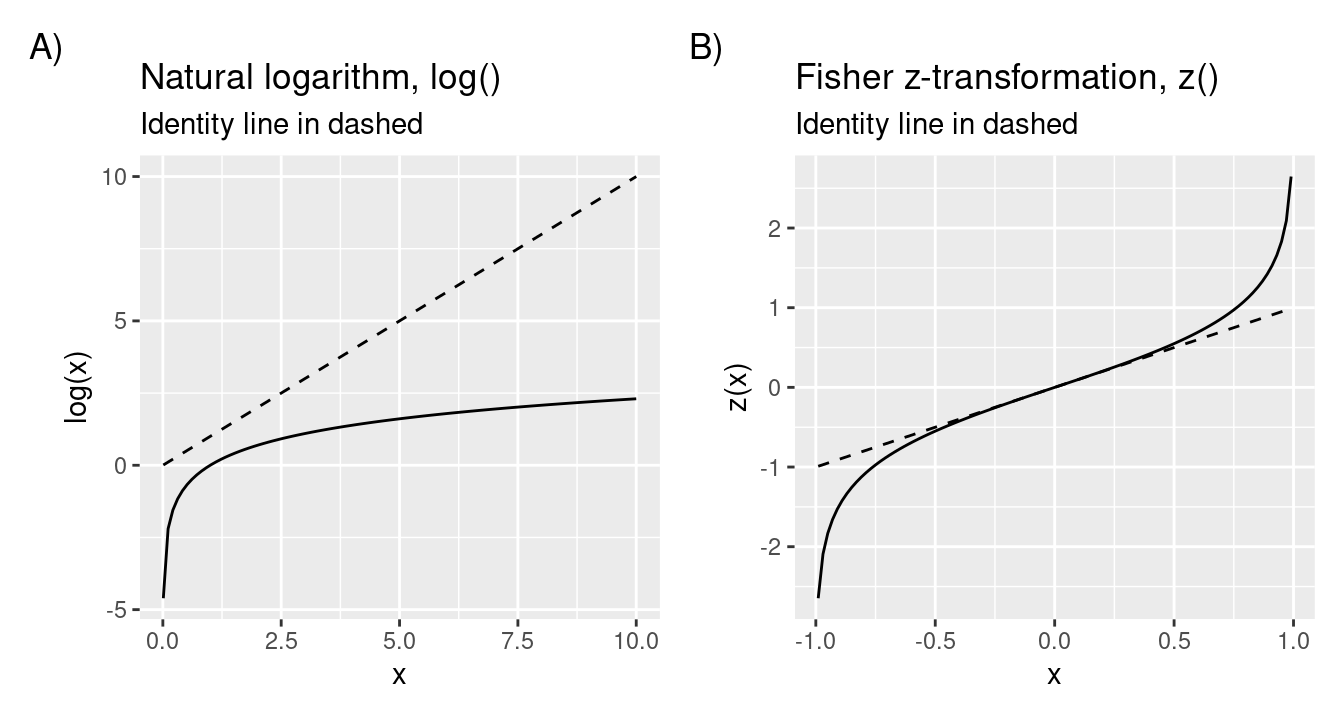
\includegraphics[width=\textwidth]{parametrization-1.png}\\
 \begin{footnotesize}
  SOURCE: The author (2021).
 \end{footnotesize}
 \label{fig:parametrization}
\end{figure}

The other parametrization option consist in estimate the elements of a
factorization or decomposition of the positive-definite matrix
\(\Sigma\). The most common is the Cholesky factorization or
decomposition \cite{cholesky}. For two competing causes of failure, a
standard Cholesky decomposition of \(\Sigma\) may be expressed as
\begin{align*}
 \Sigma = \begin{bmatrix}
           c_{1}&0&0&0\\
           c_{2}&c_{3}&0&0\\
           c_{4}&c_{5}&c_{6}&0\\
           c_{7}&c_{8}&c_{9}&c_{10}
         \end{bmatrix}\begin{bmatrix}
                       c_{1}&c_{2}&c_{4}&c_{7}\\
                       0&c_{3}&c_{5}&c_{8}\\
                       0&0&c_{6}&c_{9}\\
                       0&0&0&c_{10}
                      \end{bmatrix} = LL^{\top},
\end{align*}
where \(\{c_{i}\}_{i=1}^{10}\) are then the coefficients to be estimated.

A disadvantage in the use of a decomposition as the Cholesky is the lack
of a straightforward interpretation to the elements
\(\{c_{i}\}_{i=1}^{10}\). However, with the application of the delta
method, already implemented in TMB \cite{TMB}, it is straightforward to
get back the \(\Sigma\) elements together with its respective standard
errors. The main advantage of this parametrization, apart from the fact
that it ensures positive definiteness, is that it is computationally
simple and stable.

Just to mention another viable possibilities, we could use a modified
Cholesky decomposition \cite{modifiedcholesky} that provides a better
statistical interpretation of the decomposition elements or, we could
also parametrize the precision matrix, \(\bm{Q} = \Sigma^{-1}\). Since
we use \(\Sigma^{-1}\) in the marginal likelihood of
\autoref{eq:loglik}, parametrizing directly its inverse save us some
computations.

Besides the popularity of the Cholesky method, there is another
factorization scheme available and efficiently implemented in TMB. It is
a factorization based on a vector scale transformation of an
unstructured correlation matrix. For two competing causes of failure the
decomposition is specified in the following fashion
\[
  \Sigma = VD^{-1/2}LL^{\top}D^{-1/2}V^{\top},
\]
where
\[
 L = \begin{bmatrix}
      1&0&0&0\\
      c_{1}&1&0&0\\
      c_{2}&c_{3}&1&0\\
      c_{4}&c_{5}&c_{6}&1
     \end{bmatrix},\quad D = \text{diag}(LL^{\top})
 \quad\text{ and }\quad W = \text{diag}(\{\sigma_{i}\}_{i=1}^{4}).
\]
This scheme is based initially on the factorization of a correlation
matrix (unit diagonal) as \(D^{-1/2}LL^{\top}D^{-1/2}\). The elements
\(\{c_{i}\}_{i=1}^{6}\) to be estimated has the advantage of being
unconstrained and guarantees that the symmetry and positive definiteness
constraint is respected. The variances are scaled via the diagonal
matrix V, its elements \(\{\sigma_{i}\}_{i=1}^{4}\) are then the
standard deviations to be estimated.

% END ==================================================================
